\renewcommand{\baselinestretch}{1}\normalsize
% دانشگاه خود را وارد کنید
\university{نام دانشگاه‌تان}
% دانشکده، آموزشکده و یا پژوهشکده  خود را وارد کنید
\faculty{دانشکده محل تحصیل‌تان}
% گروه آموزشی خود را وارد کنید
\department{نام گروه آموزشی‌ که در آن تحصیل می‌کنید}
% رشته آموزشی خود را وارد کنید
\subject{نام رشته‌تان}
% گرایش خود را وارد کنید
\field{گرایش‌تان}
% عنوان پایان‌نامه را وارد کنید
\title{راهنمایی بر پایان‌نامه/رساله نویسی با تِک\;\TeX}

% نام استاد(ان) راهنما را وارد کنید
\firstsupervisor{دکتر}
%\secondsupervisor{دکتر}
% نام استاد(دان) مشاور را وارد کنید. چنانچه استاد مشاور ندارید، دستور پایین را غیرفعال کنید.
\firstadvisor{دکتر}
%\secondadvisor{دکتر}
\TSupervisor{جناب آقای دکتر}
\TAdvisor{سرکار خانم دکتر}
\TOArbiter{جناب آقای دکتر}
\TTArbiter{سرکار خانم دکتر}


% نام پژوهشگر را وارد کنید
\name{گروه دانشجویی ابوالوفا}
% نام خانوادگی پژوهشگر را وارد کنید
\surname{بوزجانی}
% تاریخ پایان‌نامه را وارد کنید
\thesisdate{فروردین ماه 1400}
\okdate{1399/6/1}
\defencedate{1399/7/1}
% کلمات کلیدی پایان‌نامه را وارد کنید
\keywords{رساله، پایان‌نامه، تک، راهنما}
% چکیده پایان‌نامه را وارد کنید
\abstract{
حداکثر در حجمی معادل با 250 تا 300 کلمه تهيه شده و شامل بيان مختصر مسئله مورد بررسی، روش تحقيق و مراحل بکار گرفته شده برای کسب و جمع آوری اطلاعات، نحوه تجزيه و تحليل و نتيجه کلی می باشد. خواننده با مطالعه چکيده بايد تشخيص دهد که رساله موجود دربرگيرنده مطالب مورد علاقه وی می باشد يا خير؟ تاريخچه و سابقه موضوع در اين قسمت ذکر نشده، بلکه در مقدمه رساله توضيح داده می شود. چکيده در يک صفحه مجزا قبل از فهرست مطالب قرار می گيرد . در بالای آن به فاصله دو سطر از حاشيه بالای صفحه در ميانه سطر عنوان پايان نامه نوشته می شود. در انتهای چکيده ميتواند کلمات کليدی مورد استفاده در پايان نامه به تعداد 5-4 واژه اضافه شود. \\
دوستان شما در این رساله سعی دارند تا شما را با یک قالب پایان‌نامه/ رساله آشنا کنند. شما با توجه به همین بسته موجود (ABThesis) و راهنمایی‌های ارائه شده در این نمونه رساله خواهید توانست با اندکی دقت ضمن یاد گرفتن اصول فنی نوشتن تحت \TeX با نگارش فنی نیز آشنا شوید، لازم به ذکر است که قالب حاضر به طور اختصاصی استانداردهای دانشگاه فردوسی را پشتیبانی می‌کند. \\
لازم به ذکر است که ما تعداد کلمات در چکیده به طور رسمی دارای محدودیت است از این‌رو ما نیز با توجه به آن فضای مربوط به چکیده‌مان را تنظیم کردیم.
}

\baselineskip=.6cm
\latinuniversity{Ferdowsi University of Mashhad}
\latinfaculty{Faculty of Mathematical Sciences}
\latinsubject{Pure Mathematics}
\latinfield{Mathematical Analysis}
\latintitle{The probabilistic powerdomain for stably compact spaces}
\firstlatinsupervisor{First Supervisor}
%\secondlatinsupervisor{Second Supervisor}
\firstlatinadvisor{First Advisor}
%\secondlatinadvisor{Second Advisor}
\latinname{English name}
\latinsurname{English family}
\latinthesisdate{2020}
\latinokdate{2020}
\latindefencedate{2020}
\latinkeywords{Probabilistic powerdomain; Stably compact space; Valuation}
\latinabstract{
This thesis reviews the one-to-one correspondence between stably compact spaces (a topological
concept covering most classes of semantic domains) and compact ordered Hausdorff spaces. The
correspondence is extended to certain classes of real-valued functions on these spaces. This is the
basis for transferring methods and results from functional analysis to the non-Hausdorff setting.
}



\pagestyle{empty}
\besm{besm}
\ftitle
%صورتجلسه بایست به امضای دانشجو و اساتید برسد و سپس اسکن آن به صورت پی‌دی‌اف در کنار فایل‌های دیگر با نام minutes ذخیره شود.

\includepdf{minutes}
\specifications
%اصالت‌نامه بایست به امضای دانشجو و اساتید راهنما برسد و سپس اسکن آن به صورت پی‌دی‌اف در کنار فایل‌های دیگر با نام originality ذخیره شود. فایل خام آن را می‌توانید از پوشه other بردارید.
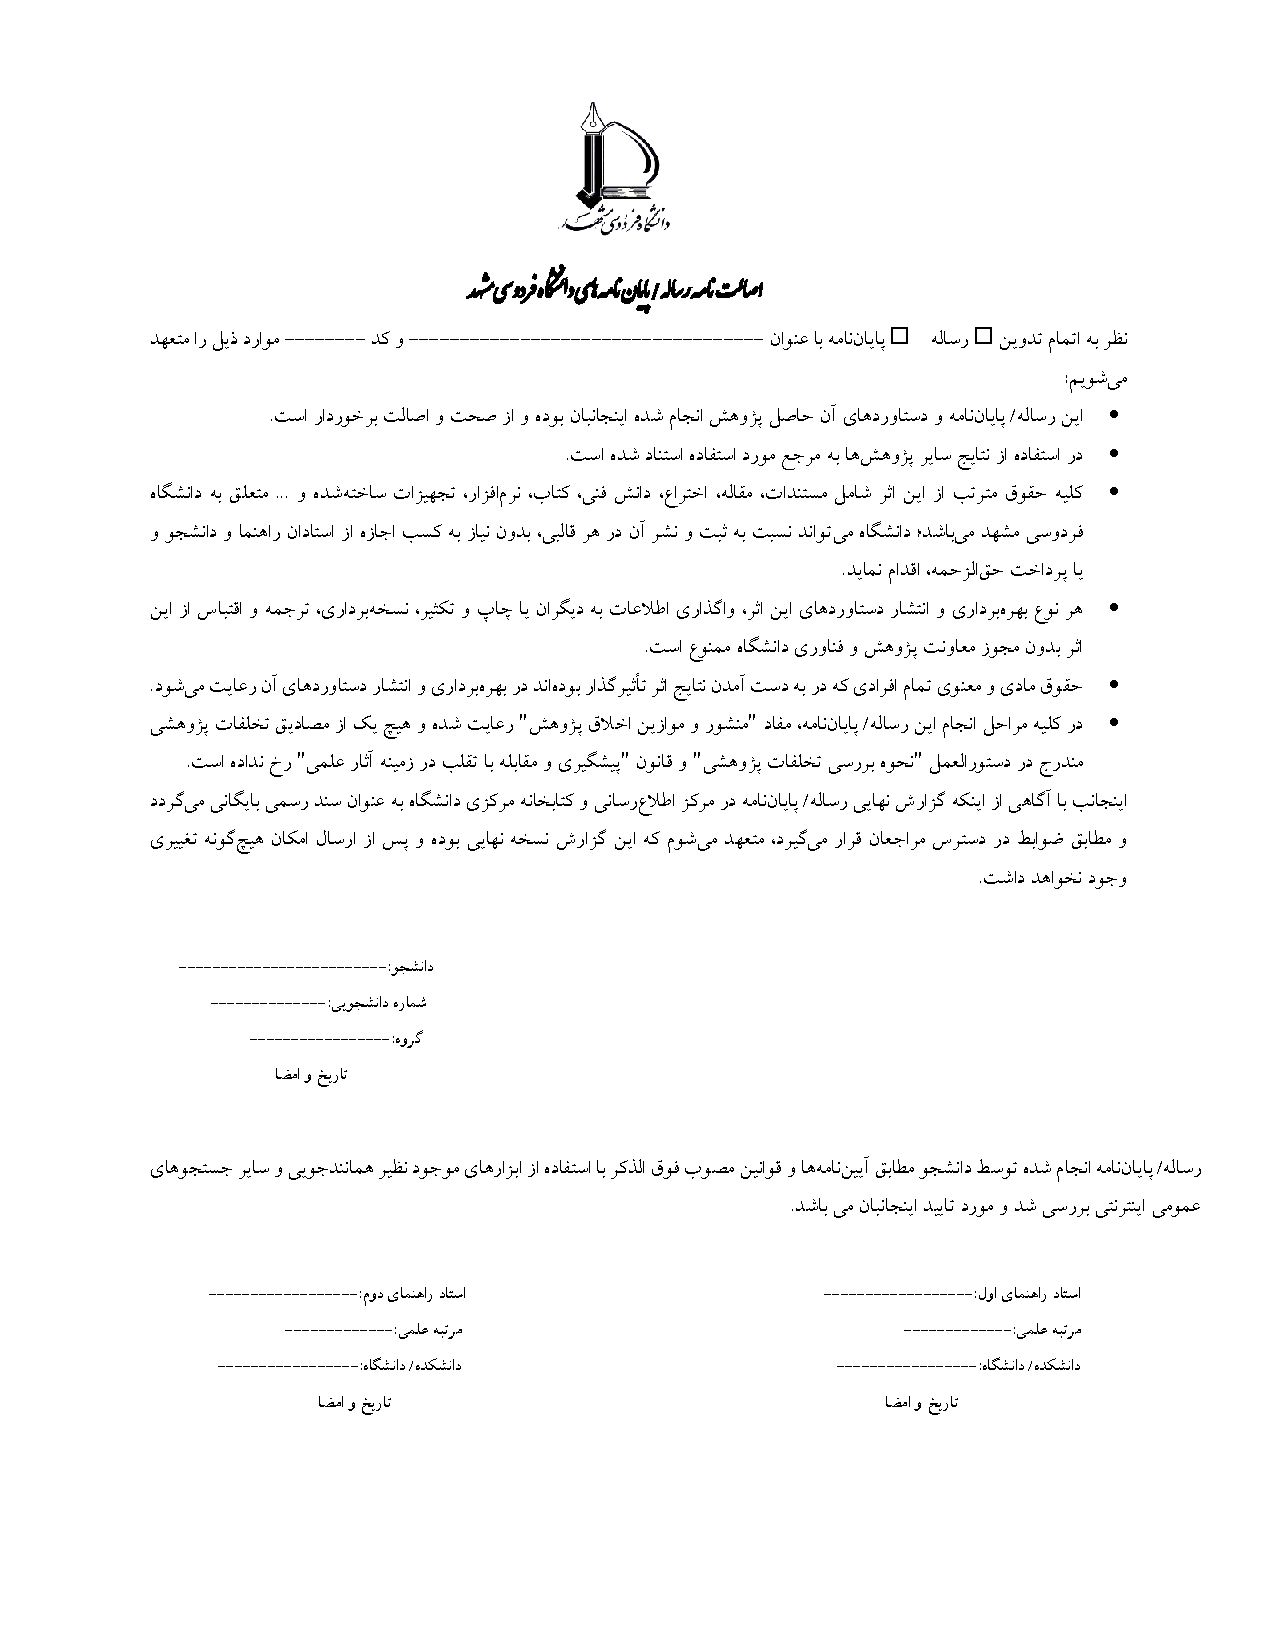
\includepdf{originality}
\presentation{1}{تقدیم به }{...}{که ...}
\praise{1}{هوالعلیم،}{به نام حق که ...\\}{می‌کوش به هر ورق که خوانی \hspace*{\fill} تا معنی آن تمام دانی}
\thanks{1}{سپاس‌گزاری}{سپاس خداوند بلندمرتبه\\}{نام}‮‮



%در صورتی که مایل به استفاده از فهرست نماد هستید عبارت‌های مربوط به محیط comment را در خط بعد و خط آخر این فایل حذف کنید. لازم به ذکر است که از دو نوع فهرست نماد هر کدام را که مایل هستید می‌توانید استفاده کنید و دیگری را بایست حذف نمایید. 
\begin{comment}
\newpage
\begin{center}
\tos{فهرست نمادها و علائم ریاضی}{%
\srow{جمع}{$\sum$}
\srow{ضرب}{$\prod$}
\srow{تقسیم}{$/$}
}{2} 
\end{center}

\begin{center}
\tos{فهرست نمادها و علائم ریاضی}{%
\srow{جمع}{$\sum$}{s1}
\srow{ضرب}{$\prod$}{s1}
\srow{تقسیم}{$/$}{s1}
}{3}
\end{center}
برای این‌که فهرست نمادها را به کارتان اضافه کنید کافی‌ست بعد از انتخاب یکی از دو جدول فوق بقیه سطرها را به انتخاب خودتان تکمیل کنید. شاید اساسی‌ترین نکته دقت در به کار بردن فهرست سه ستونه است که برای استفاده از آن شما باید در جایی که نماد برای بار اول به کار برده می‌شود از دستور label استفاده کنید و برای تکمیل جدول فقط پارامتری که  هنگام استفاده از label استفاده کرده‌اید را بنویسید.
$\sum\label{s1}$
\pagebreak
\end{comment}